\documentclass{article}
\usepackage{graphicx}

\begin{document}
\title{\LARGE Assignment 10}
\author{Jianqiang Du\\\\017547307}
\maketitle

\section{Consider the 101 x 3 world shown in Figure 1. In the start state the agent has a choice of two deterministic actions, Up or Down, but in the other states the agent has one deterministic action, Right. Assuming a discounted reward function.}
	\begin{itemize}
		\item[(a)]Compute the utility of each action as a function of $\gamma$.
		\begin{itemize}
			\item[Answer:]UP: $U = \sum_{t=0}^{101}\gamma ^tR(S_t)\\=0+\gamma^1R(S_1)+\sum_{t=2}^{100}\gamma ^tR(S_t)+\gamma^{101}R(S_{101})\\=50\gamma - \sum_{t=2}^{100}\gamma ^t + \gamma^{101}\\=50\gamma - \gamma^2\frac{1-\gamma^{99}}{1-\gamma}+\gamma^{101}$\\DOWN: $U = \sum_{t=0}^{101}\gamma ^tR(S_t)\\=0+\gamma^1R(S_1)+\sum_{t=2}^{100}\gamma ^tR(S_t)+\gamma^{101}R(S_{101})\\=-50\gamma + \sum_{t=2}^{100}\gamma ^t - \gamma^{101}\\=-50\gamma + \gamma^2\frac{1-\gamma^{99}}{1-\gamma}-\gamma^{101}$
		\end{itemize}
		\item[(b)]Draw the utility of each action for the range 0 $\leq \gamma \leq$ 1 using \textbf{Matlab} of your familiar numerical analysis software.
		\begin{itemize}
			\item[Answer:]See below.
		\end{itemize}
		\begin{figure}[h!]
			\centering
			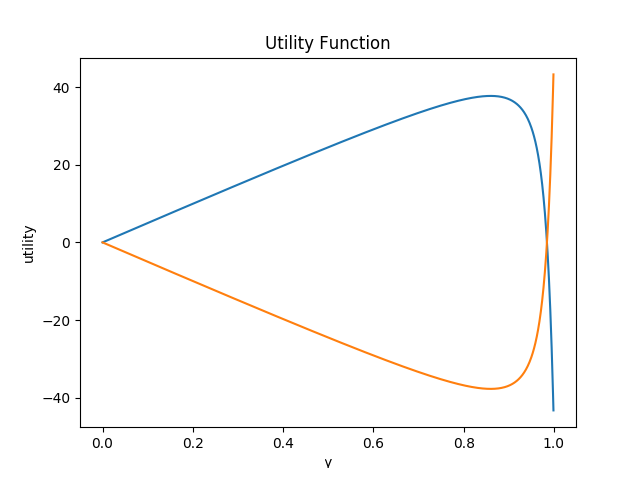
\includegraphics[width=\textwidth]{utility_vs_gamma.png}
			\title{1. (b)}
		\end{figure}
		\item[(c)]For $\gamma$ = $\frac{1}{2}$, which action is recommend? Why?
		\begin{itemize}
			\item[Answer:]UP is recommended because uitility of UP is greater than utility of DOWN according to (b).
		\end{itemize}
	\end{itemize}
	\begin{figure}[h!]
		\centering
		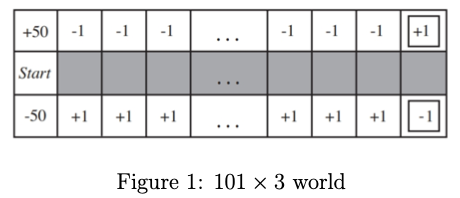
\includegraphics[width=0.65\textwidth]{fig1.png}
	\end{figure}
\section{Consider the following data set comprised of three binary input attributes ($A_1$, $A_2$, and $A_3$) and one binary output:}
	\begin{itemize}
		\item[(a)]Computer \textit{Gain}($A_1$).
			\begin{itemize}
				\item[Answer:]$Gain(A_1)=B(\frac{2}{5})-\frac{4}{5}B(\frac{2}{4})-\frac{1}{5}B(\frac{0}{1})=0.1710$
			\end{itemize}
		\item[(b)]Computer \textit{Gain}($A_2$).
			\begin{itemize}
				\item[Answer:]$Gain(A_2)=B(\frac{2}{5})-\frac{3}{5}B(\frac{2}{3})-\frac{2}{5}B(\frac{0}{2})=0.4200$
			\end{itemize}
		\item[(c)]Computer \textit{Gain}($A_3$).
			\begin{itemize}
				\item[Answer:]$Gain(A_3)=B(\frac{2}{5})-\frac{2}{5}B(\frac{1}{2})-\frac{3}{5}B(\frac{1}{3})=0.0200$
			\end{itemize}
	\end{itemize}
	\begin{figure}[h!]
		\centering
		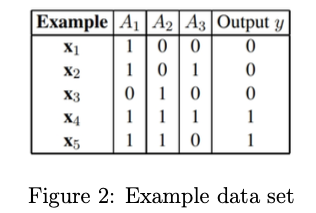
\includegraphics[width=0.5\textwidth]{fig2.png}
	\end{figure}
	
\section{Consider the XOR function of three binary input attributes ($A_1$, $A_2$, and $A_3$), which produces the value 1 if and only if an odd number of the three input attributes has value 1. Draw a minimal-sized decision tree for the three-input XOR function.}
	\begin{figure}[h!]
	\centering
	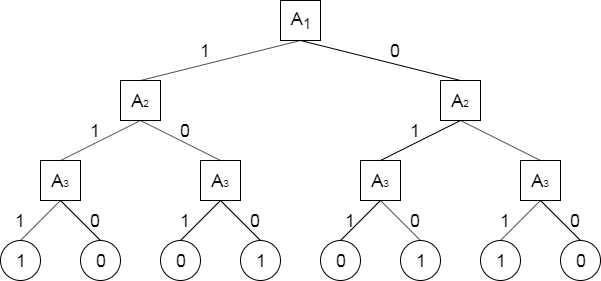
\includegraphics[width=\textwidth]{decision_tree.png}
	\end{figure}
\end{document}